  
As explained in the dataset section, we divide the dataset into different eras and analysed the data using proposed method. One can see in \ref{fig:Overall_network} the evolution of the network between different sites. Mycenae wasn't the prominant center until 1300BC. The city is networked to may places as time evolves. Berbati became the prominant city after 1000 bc (?? citation), which can be seen from the network.
We also combine the data from all the eras and see how different sites are connected. 


\begin{figure}
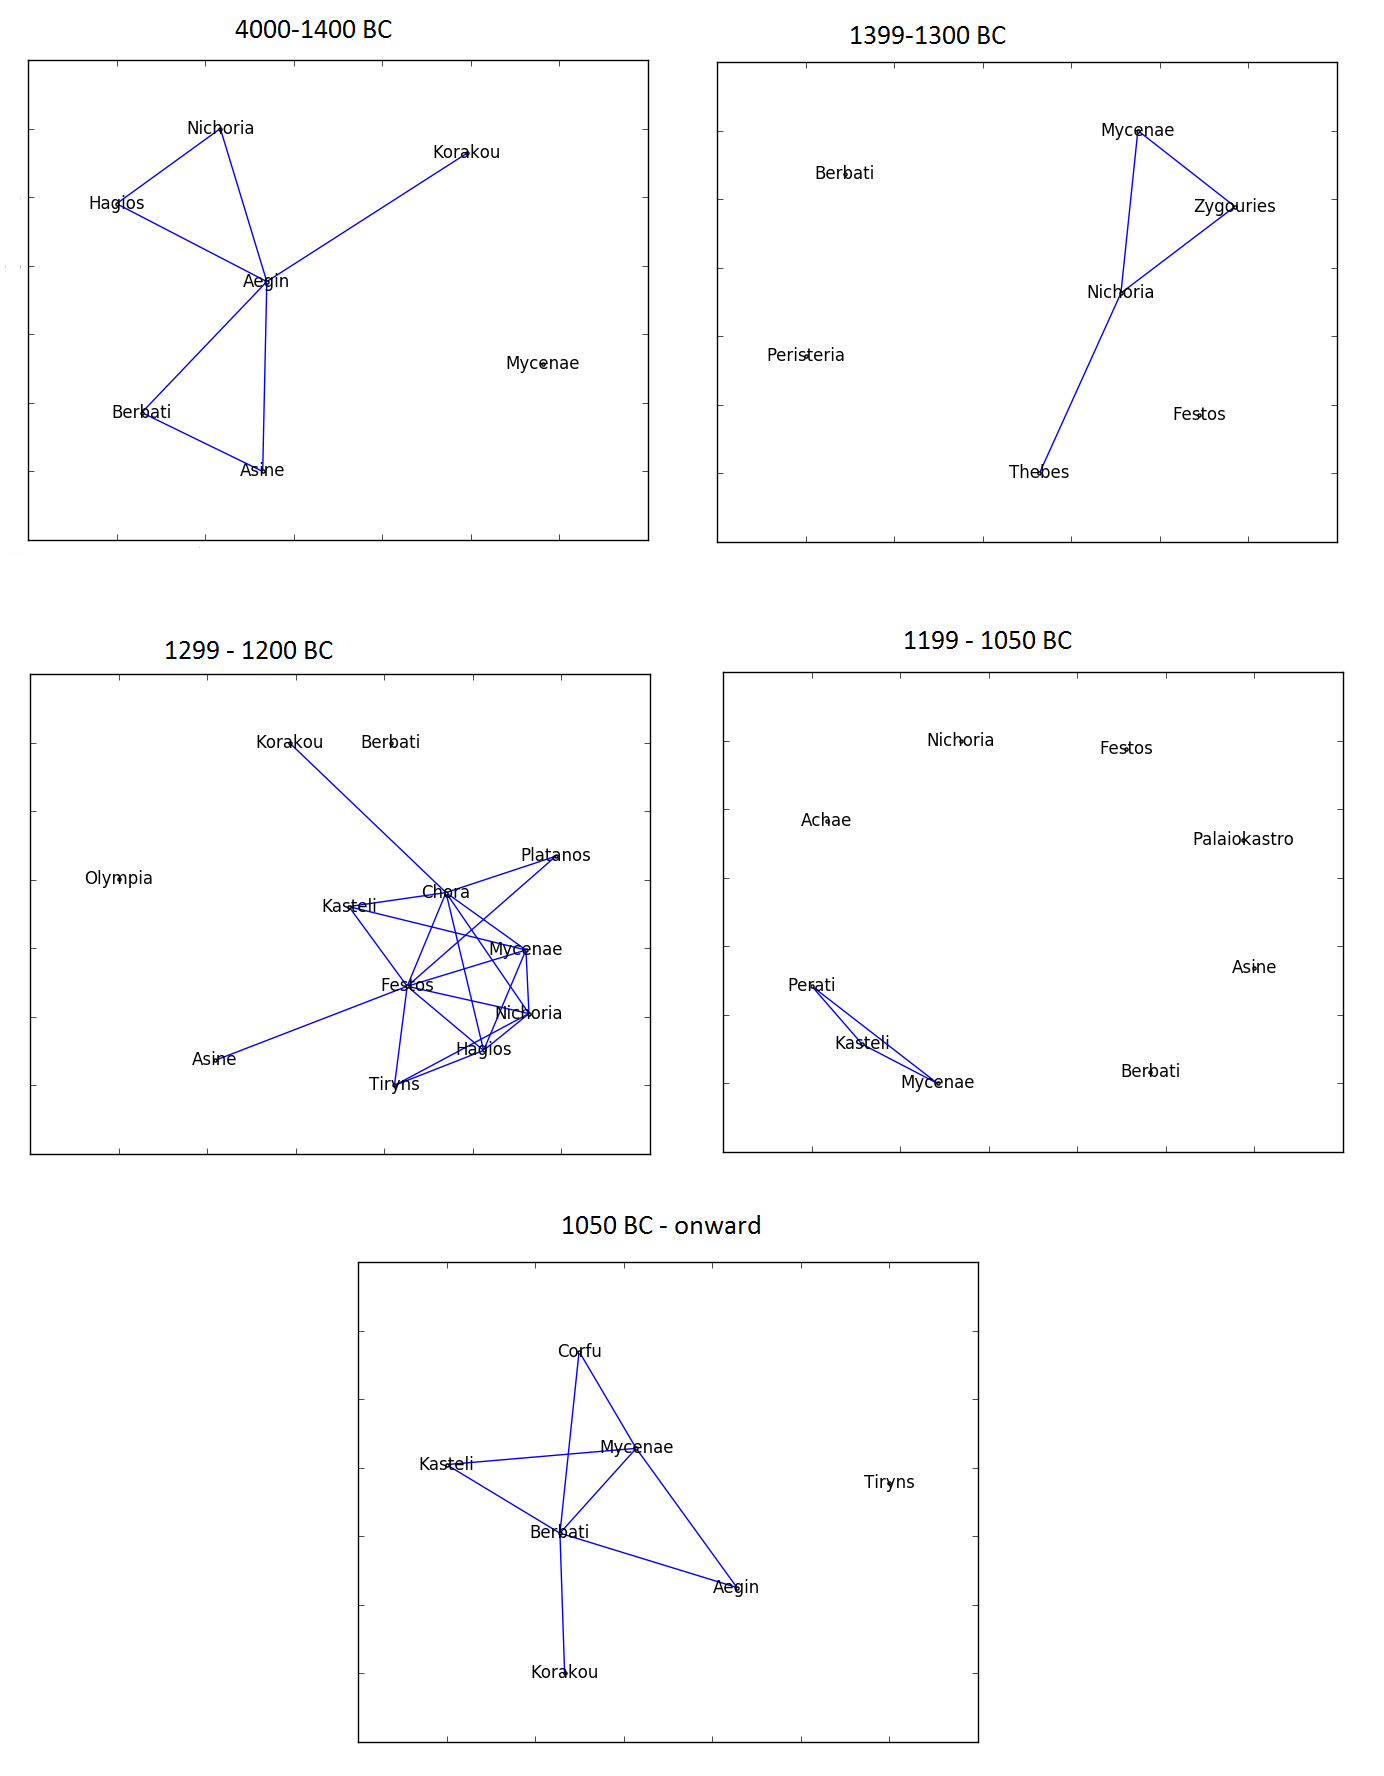
\includegraphics[width=\textwidth]{Network_evolution.png}
\caption{Evolution of networks of the Archaeological sites}
\end{figure}


\begin{figure}
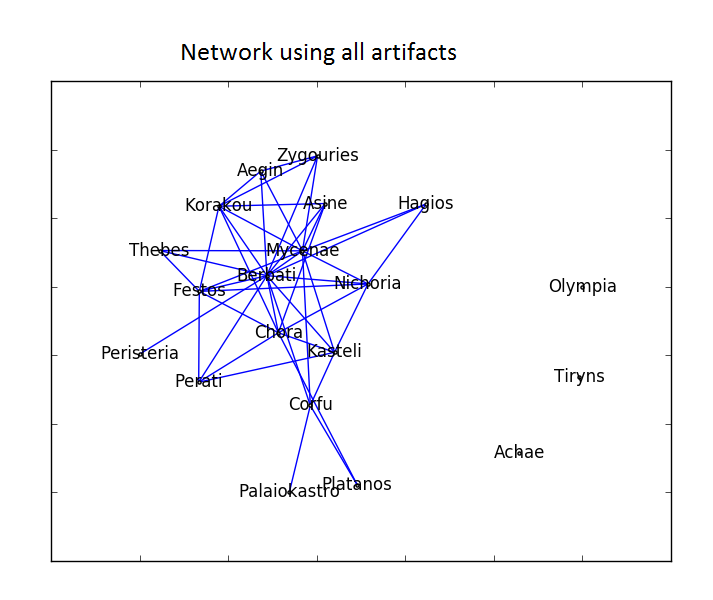
\includegraphics[width=\textwidth]{Overall_Network.png}
\caption{Overall network of the Archaeological sites}
\end{figure}
